% Options for packages loaded elsewhere
\PassOptionsToPackage{unicode}{hyperref}
\PassOptionsToPackage{hyphens}{url}
%
\documentclass[
]{article}
\usepackage{amsmath,amssymb}
\usepackage{lmodern}
\usepackage{iftex}
\ifPDFTeX
  \usepackage[T1]{fontenc}
  \usepackage[utf8]{inputenc}
  \usepackage{textcomp} % provide euro and other symbols
\else % if luatex or xetex
  \usepackage{unicode-math}
  \defaultfontfeatures{Scale=MatchLowercase}
  \defaultfontfeatures[\rmfamily]{Ligatures=TeX,Scale=1}
\fi
% Use upquote if available, for straight quotes in verbatim environments
\IfFileExists{upquote.sty}{\usepackage{upquote}}{}
\IfFileExists{microtype.sty}{% use microtype if available
  \usepackage[]{microtype}
  \UseMicrotypeSet[protrusion]{basicmath} % disable protrusion for tt fonts
}{}
\makeatletter
\@ifundefined{KOMAClassName}{% if non-KOMA class
  \IfFileExists{parskip.sty}{%
    \usepackage{parskip}
  }{% else
    \setlength{\parindent}{0pt}
    \setlength{\parskip}{6pt plus 2pt minus 1pt}}
}{% if KOMA class
  \KOMAoptions{parskip=half}}
\makeatother
\usepackage{xcolor}
\usepackage[margin=1in]{geometry}
\usepackage{color}
\usepackage{fancyvrb}
\newcommand{\VerbBar}{|}
\newcommand{\VERB}{\Verb[commandchars=\\\{\}]}
\DefineVerbatimEnvironment{Highlighting}{Verbatim}{commandchars=\\\{\}}
% Add ',fontsize=\small' for more characters per line
\usepackage{framed}
\definecolor{shadecolor}{RGB}{248,248,248}
\newenvironment{Shaded}{\begin{snugshade}}{\end{snugshade}}
\newcommand{\AlertTok}[1]{\textcolor[rgb]{0.94,0.16,0.16}{#1}}
\newcommand{\AnnotationTok}[1]{\textcolor[rgb]{0.56,0.35,0.01}{\textbf{\textit{#1}}}}
\newcommand{\AttributeTok}[1]{\textcolor[rgb]{0.77,0.63,0.00}{#1}}
\newcommand{\BaseNTok}[1]{\textcolor[rgb]{0.00,0.00,0.81}{#1}}
\newcommand{\BuiltInTok}[1]{#1}
\newcommand{\CharTok}[1]{\textcolor[rgb]{0.31,0.60,0.02}{#1}}
\newcommand{\CommentTok}[1]{\textcolor[rgb]{0.56,0.35,0.01}{\textit{#1}}}
\newcommand{\CommentVarTok}[1]{\textcolor[rgb]{0.56,0.35,0.01}{\textbf{\textit{#1}}}}
\newcommand{\ConstantTok}[1]{\textcolor[rgb]{0.00,0.00,0.00}{#1}}
\newcommand{\ControlFlowTok}[1]{\textcolor[rgb]{0.13,0.29,0.53}{\textbf{#1}}}
\newcommand{\DataTypeTok}[1]{\textcolor[rgb]{0.13,0.29,0.53}{#1}}
\newcommand{\DecValTok}[1]{\textcolor[rgb]{0.00,0.00,0.81}{#1}}
\newcommand{\DocumentationTok}[1]{\textcolor[rgb]{0.56,0.35,0.01}{\textbf{\textit{#1}}}}
\newcommand{\ErrorTok}[1]{\textcolor[rgb]{0.64,0.00,0.00}{\textbf{#1}}}
\newcommand{\ExtensionTok}[1]{#1}
\newcommand{\FloatTok}[1]{\textcolor[rgb]{0.00,0.00,0.81}{#1}}
\newcommand{\FunctionTok}[1]{\textcolor[rgb]{0.00,0.00,0.00}{#1}}
\newcommand{\ImportTok}[1]{#1}
\newcommand{\InformationTok}[1]{\textcolor[rgb]{0.56,0.35,0.01}{\textbf{\textit{#1}}}}
\newcommand{\KeywordTok}[1]{\textcolor[rgb]{0.13,0.29,0.53}{\textbf{#1}}}
\newcommand{\NormalTok}[1]{#1}
\newcommand{\OperatorTok}[1]{\textcolor[rgb]{0.81,0.36,0.00}{\textbf{#1}}}
\newcommand{\OtherTok}[1]{\textcolor[rgb]{0.56,0.35,0.01}{#1}}
\newcommand{\PreprocessorTok}[1]{\textcolor[rgb]{0.56,0.35,0.01}{\textit{#1}}}
\newcommand{\RegionMarkerTok}[1]{#1}
\newcommand{\SpecialCharTok}[1]{\textcolor[rgb]{0.00,0.00,0.00}{#1}}
\newcommand{\SpecialStringTok}[1]{\textcolor[rgb]{0.31,0.60,0.02}{#1}}
\newcommand{\StringTok}[1]{\textcolor[rgb]{0.31,0.60,0.02}{#1}}
\newcommand{\VariableTok}[1]{\textcolor[rgb]{0.00,0.00,0.00}{#1}}
\newcommand{\VerbatimStringTok}[1]{\textcolor[rgb]{0.31,0.60,0.02}{#1}}
\newcommand{\WarningTok}[1]{\textcolor[rgb]{0.56,0.35,0.01}{\textbf{\textit{#1}}}}
\usepackage{longtable,booktabs,array}
\usepackage{calc} % for calculating minipage widths
% Correct order of tables after \paragraph or \subparagraph
\usepackage{etoolbox}
\makeatletter
\patchcmd\longtable{\par}{\if@noskipsec\mbox{}\fi\par}{}{}
\makeatother
% Allow footnotes in longtable head/foot
\IfFileExists{footnotehyper.sty}{\usepackage{footnotehyper}}{\usepackage{footnote}}
\makesavenoteenv{longtable}
\usepackage{graphicx}
\makeatletter
\def\maxwidth{\ifdim\Gin@nat@width>\linewidth\linewidth\else\Gin@nat@width\fi}
\def\maxheight{\ifdim\Gin@nat@height>\textheight\textheight\else\Gin@nat@height\fi}
\makeatother
% Scale images if necessary, so that they will not overflow the page
% margins by default, and it is still possible to overwrite the defaults
% using explicit options in \includegraphics[width, height, ...]{}
\setkeys{Gin}{width=\maxwidth,height=\maxheight,keepaspectratio}
% Set default figure placement to htbp
\makeatletter
\def\fps@figure{htbp}
\makeatother
\setlength{\emergencystretch}{3em} % prevent overfull lines
\providecommand{\tightlist}{%
  \setlength{\itemsep}{0pt}\setlength{\parskip}{0pt}}
\setcounter{secnumdepth}{-\maxdimen} % remove section numbering
\ifLuaTeX
  \usepackage{selnolig}  % disable illegal ligatures
\fi
\IfFileExists{bookmark.sty}{\usepackage{bookmark}}{\usepackage{hyperref}}
\IfFileExists{xurl.sty}{\usepackage{xurl}}{} % add URL line breaks if available
\urlstyle{same} % disable monospaced font for URLs
\hypersetup{
  pdftitle={Bishop Lab 3},
  pdfauthor={Erica Bishop},
  hidelinks,
  pdfcreator={LaTeX via pandoc}}

\title{Bishop Lab 3}
\author{Erica Bishop}
\date{2023-01-25}

\begin{document}
\maketitle

\hypertarget{lab-3-predicting-the-age-of-abalone}{%
\subsection{Lab 3: Predicting the age of
abalone}\label{lab-3-predicting-the-age-of-abalone}}

Abalones are marine snails. Their flesh is widely considered to be a
desirable food, and is consumed raw or cooked by a variety of cultures.
The age of abalone is determined by cutting the shell through the cone,
staining it, and counting the number of rings through a microscope -- a
boring and time-consuming task. Other measurements, which are easier to
obtain, are used to predict the age.

The data set provided includes variables related to the sex, physical
dimensions of the shell, and various weight measurements, along with the
number of rings in the shell. Number of rings is the stand-in here for
age.

\hypertarget{data-exploration}{%
\subsubsection{Data Exploration}\label{data-exploration}}

Pull the abalone data from Github and take a look at it.

\begin{Shaded}
\begin{Highlighting}[]
\NormalTok{abdat }\OtherTok{\textless{}{-}} \FunctionTok{read\_csv}\NormalTok{(}\AttributeTok{file =} \StringTok{"https://raw.githubusercontent.com/MaRo406/eds{-}232{-}machine{-}learning/main/data/abalone{-}data.csv"}\NormalTok{)}
\end{Highlighting}
\end{Shaded}

\begin{verbatim}
## New names:
## Rows: 4177 Columns: 10
## -- Column specification
## -------------------------------------------------------- Delimiter: "," chr
## (1): Sex dbl (9): ...1, Length, Diameter, Height, Whole_weight, Shucked_weight,
## Visce...
## i Use `spec()` to retrieve the full column specification for this data. i
## Specify the column types or set `show_col_types = FALSE` to quiet this message.
## * `` -> `...1`
\end{verbatim}

\begin{Shaded}
\begin{Highlighting}[]
\FunctionTok{glimpse}\NormalTok{(abdat)}
\end{Highlighting}
\end{Shaded}

\begin{verbatim}
## Rows: 4,177
## Columns: 10
## $ ...1           <dbl> 1, 2, 3, 4, 5, 6, 7, 8, 9, 10, 11, 12, 13, 14, 15, 16, ~
## $ Sex            <chr> "M", "M", "F", "M", "I", "I", "F", "F", "M", "F", "F", ~
## $ Length         <dbl> 0.455, 0.350, 0.530, 0.440, 0.330, 0.425, 0.530, 0.545,~
## $ Diameter       <dbl> 0.365, 0.265, 0.420, 0.365, 0.255, 0.300, 0.415, 0.425,~
## $ Height         <dbl> 0.095, 0.090, 0.135, 0.125, 0.080, 0.095, 0.150, 0.125,~
## $ Whole_weight   <dbl> 0.5140, 0.2255, 0.6770, 0.5160, 0.2050, 0.3515, 0.7775,~
## $ Shucked_weight <dbl> 0.2245, 0.0995, 0.2565, 0.2155, 0.0895, 0.1410, 0.2370,~
## $ Viscera_weight <dbl> 0.1010, 0.0485, 0.1415, 0.1140, 0.0395, 0.0775, 0.1415,~
## $ Shell_weight   <dbl> 0.150, 0.070, 0.210, 0.155, 0.055, 0.120, 0.330, 0.260,~
## $ Rings          <dbl> 15, 7, 9, 10, 7, 8, 20, 16, 9, 19, 14, 10, 11, 10, 10, ~
\end{verbatim}

\begin{Shaded}
\begin{Highlighting}[]
\NormalTok{skimr}\SpecialCharTok{::}\FunctionTok{skim}\NormalTok{(abdat) }\CommentTok{\#check out completeness of data}
\end{Highlighting}
\end{Shaded}

\begin{longtable}[]{@{}ll@{}}
\caption{Data summary}\tabularnewline
\toprule()
\endhead
Name & abdat \\
Number of rows & 4177 \\
Number of columns & 10 \\
\_\_\_\_\_\_\_\_\_\_\_\_\_\_\_\_\_\_\_\_\_\_\_ & \\
Column type frequency: & \\
character & 1 \\
numeric & 9 \\
\_\_\_\_\_\_\_\_\_\_\_\_\_\_\_\_\_\_\_\_\_\_\_\_ & \\
Group variables & None \\
\bottomrule()
\end{longtable}

\textbf{Variable type: character}

\begin{longtable}[]{@{}
  >{\raggedright\arraybackslash}p{(\columnwidth - 14\tabcolsep) * \real{0.1944}}
  >{\raggedleft\arraybackslash}p{(\columnwidth - 14\tabcolsep) * \real{0.1389}}
  >{\raggedleft\arraybackslash}p{(\columnwidth - 14\tabcolsep) * \real{0.1944}}
  >{\raggedleft\arraybackslash}p{(\columnwidth - 14\tabcolsep) * \real{0.0556}}
  >{\raggedleft\arraybackslash}p{(\columnwidth - 14\tabcolsep) * \real{0.0556}}
  >{\raggedleft\arraybackslash}p{(\columnwidth - 14\tabcolsep) * \real{0.0833}}
  >{\raggedleft\arraybackslash}p{(\columnwidth - 14\tabcolsep) * \real{0.1250}}
  >{\raggedleft\arraybackslash}p{(\columnwidth - 14\tabcolsep) * \real{0.1528}}@{}}
\toprule()
\begin{minipage}[b]{\linewidth}\raggedright
skim\_variable
\end{minipage} & \begin{minipage}[b]{\linewidth}\raggedleft
n\_missing
\end{minipage} & \begin{minipage}[b]{\linewidth}\raggedleft
complete\_rate
\end{minipage} & \begin{minipage}[b]{\linewidth}\raggedleft
min
\end{minipage} & \begin{minipage}[b]{\linewidth}\raggedleft
max
\end{minipage} & \begin{minipage}[b]{\linewidth}\raggedleft
empty
\end{minipage} & \begin{minipage}[b]{\linewidth}\raggedleft
n\_unique
\end{minipage} & \begin{minipage}[b]{\linewidth}\raggedleft
whitespace
\end{minipage} \\
\midrule()
\endhead
Sex & 0 & 1 & 1 & 1 & 0 & 3 & 0 \\
\bottomrule()
\end{longtable}

\textbf{Variable type: numeric}

\begin{longtable}[]{@{}
  >{\raggedright\arraybackslash}p{(\columnwidth - 20\tabcolsep) * \real{0.1531}}
  >{\raggedleft\arraybackslash}p{(\columnwidth - 20\tabcolsep) * \real{0.1020}}
  >{\raggedleft\arraybackslash}p{(\columnwidth - 20\tabcolsep) * \real{0.1429}}
  >{\raggedleft\arraybackslash}p{(\columnwidth - 20\tabcolsep) * \real{0.0816}}
  >{\raggedleft\arraybackslash}p{(\columnwidth - 20\tabcolsep) * \real{0.0816}}
  >{\raggedleft\arraybackslash}p{(\columnwidth - 20\tabcolsep) * \real{0.0510}}
  >{\raggedleft\arraybackslash}p{(\columnwidth - 20\tabcolsep) * \real{0.0816}}
  >{\raggedleft\arraybackslash}p{(\columnwidth - 20\tabcolsep) * \real{0.0816}}
  >{\raggedleft\arraybackslash}p{(\columnwidth - 20\tabcolsep) * \real{0.0816}}
  >{\raggedleft\arraybackslash}p{(\columnwidth - 20\tabcolsep) * \real{0.0816}}
  >{\raggedright\arraybackslash}p{(\columnwidth - 20\tabcolsep) * \real{0.0612}}@{}}
\toprule()
\begin{minipage}[b]{\linewidth}\raggedright
skim\_variable
\end{minipage} & \begin{minipage}[b]{\linewidth}\raggedleft
n\_missing
\end{minipage} & \begin{minipage}[b]{\linewidth}\raggedleft
complete\_rate
\end{minipage} & \begin{minipage}[b]{\linewidth}\raggedleft
mean
\end{minipage} & \begin{minipage}[b]{\linewidth}\raggedleft
sd
\end{minipage} & \begin{minipage}[b]{\linewidth}\raggedleft
p0
\end{minipage} & \begin{minipage}[b]{\linewidth}\raggedleft
p25
\end{minipage} & \begin{minipage}[b]{\linewidth}\raggedleft
p50
\end{minipage} & \begin{minipage}[b]{\linewidth}\raggedleft
p75
\end{minipage} & \begin{minipage}[b]{\linewidth}\raggedleft
p100
\end{minipage} & \begin{minipage}[b]{\linewidth}\raggedright
hist
\end{minipage} \\
\midrule()
\endhead
\ldots1 & 0 & 1 & 2089.00 & 1205.94 & 1.00 & 1045.00 & 2089.00 & 3133.00
& 4177.00 & ▇▇▇▇▇ \\
Length & 0 & 1 & 0.52 & 0.12 & 0.07 & 0.45 & 0.54 & 0.62 & 0.81 &
▁▂▅▇▂ \\
Diameter & 0 & 1 & 0.41 & 0.10 & 0.06 & 0.35 & 0.42 & 0.48 & 0.65 &
▁▂▆▇▁ \\
Height & 0 & 1 & 0.14 & 0.04 & 0.00 & 0.12 & 0.14 & 0.16 & 1.13 &
▇▁▁▁▁ \\
Whole\_weight & 0 & 1 & 0.83 & 0.49 & 0.00 & 0.44 & 0.80 & 1.15 & 2.83 &
▇▇▅▁▁ \\
Shucked\_weight & 0 & 1 & 0.36 & 0.22 & 0.00 & 0.19 & 0.34 & 0.50 & 1.49
& ▇▇▂▁▁ \\
Viscera\_weight & 0 & 1 & 0.18 & 0.11 & 0.00 & 0.09 & 0.17 & 0.25 & 0.76
& ▇▇▂▁▁ \\
Shell\_weight & 0 & 1 & 0.24 & 0.14 & 0.00 & 0.13 & 0.23 & 0.33 & 1.00 &
▇▇▂▁▁ \\
Rings & 0 & 1 & 9.93 & 3.22 & 1.00 & 8.00 & 9.00 & 11.00 & 29.00 &
▁▇▂▁▁ \\
\bottomrule()
\end{longtable}

\begin{Shaded}
\begin{Highlighting}[]
\CommentTok{\#drop the index column}
\NormalTok{abdat }\OtherTok{\textless{}{-}}\NormalTok{ abdat }\SpecialCharTok{|\textgreater{}} 
  \FunctionTok{select}\NormalTok{(}\SpecialCharTok{!}\StringTok{"...1"}\NormalTok{)}

\CommentTok{\#take a look at distribution of rings (to see if transformation might be needed)}
\CommentTok{\# ggplot(data = abdat,}
\CommentTok{\#        aes(x = Rings)) +}
\CommentTok{\#   geom\_histogram()}

\CommentTok{\#distribution looks normal enough}
\CommentTok{\# commented out for conciseness of knitted output}
\end{Highlighting}
\end{Shaded}

\hypertarget{data-splitting}{%
\subsubsection{Data Splitting}\label{data-splitting}}

\begin{itemize}
\tightlist
\item
  \textbf{\emph{Question 1}}. Split the data into training and test
  sets. Use a 70/30 training/test split.
\end{itemize}

We'll follow our text book's lead and use the caret package in our
approach to this task. We will use the glmnet package in order to
perform ridge regression and the lasso. The main function in this
package is glmnet(), which can be used to fit ridge regression models,
lasso models, and more. In particular, we must pass in an x matrix of
predictors as well as a y outcome vector , and we do not use the y∼x
syntax.

\begin{Shaded}
\begin{Highlighting}[]
\CommentTok{\#set seed for reproducibility}
\FunctionTok{set.seed}\NormalTok{(}\DecValTok{123}\NormalTok{)}

\NormalTok{ab\_split }\OtherTok{\textless{}{-}} \FunctionTok{initial\_split}\NormalTok{(abdat, }\AttributeTok{prop =}\NormalTok{ .}\DecValTok{7}\NormalTok{, }\CommentTok{\#set up split function for 70/30 split}
                          \AttributeTok{strata =} \StringTok{"Rings"}\NormalTok{) }\CommentTok{\#specify strata to outcome variable}

\CommentTok{\#assign training and test data sets}
\NormalTok{ab\_train }\OtherTok{\textless{}{-}} \FunctionTok{training}\NormalTok{(ab\_split)}
\NormalTok{ab\_test }\OtherTok{\textless{}{-}} \FunctionTok{testing}\NormalTok{(ab\_split)}
\end{Highlighting}
\end{Shaded}

\hypertarget{fit-a-ridge-regression-model}{%
\subsubsection{Fit a ridge regression
model}\label{fit-a-ridge-regression-model}}

\textbf{\emph{Question 2}}. Use the model.matrix() function to create a
predictor matrix, x, and assign the Rings variable to an outcome vector,
y.

\begin{Shaded}
\begin{Highlighting}[]
\CommentTok{\#Create training feature matrix}

\NormalTok{X }\OtherTok{\textless{}{-}} \FunctionTok{model.matrix}\NormalTok{(Rings }\SpecialCharTok{\textasciitilde{}}\NormalTok{., ab\_train) }
\NormalTok{X }\OtherTok{\textless{}{-}}\NormalTok{ X[,}\SpecialCharTok{{-}}\DecValTok{1}\NormalTok{] }\CommentTok{\#remove intercept column}

\CommentTok{\#assign y to outcome variable}
\NormalTok{Y }\OtherTok{\textless{}{-}}\NormalTok{ ab\_train}\SpecialCharTok{$}\NormalTok{Rings}
\end{Highlighting}
\end{Shaded}

\textbf{\emph{Question 3}}. Fit a ridge model (controlled by the alpha
parameter) using the glmnet() function. Make a plot showing how the
estimated coefficients change with lambda. (Hint: You can call plot()
directly on the glmnet() objects).

\begin{Shaded}
\begin{Highlighting}[]
\CommentTok{\#fit a ridge model with alpha = 0}
\NormalTok{ridge\_mod }\OtherTok{\textless{}{-}} \FunctionTok{glmnet}\NormalTok{(}\AttributeTok{x =}\NormalTok{ X,}
                    \AttributeTok{y =}\NormalTok{ Y,}
                    \AttributeTok{alpha =} \DecValTok{0}\NormalTok{)}

\CommentTok{\#plot}
\FunctionTok{plot}\NormalTok{(ridge\_mod, }\AttributeTok{xvar =} \StringTok{"lambda"}\NormalTok{)}
\end{Highlighting}
\end{Shaded}

\includegraphics{Lab3_files/figure-latex/unnamed-chunk-3-1.pdf}

\hypertarget{using-k-fold-cross-validation-resampling-and-tuning-our-models}{%
\subsubsection{\texorpdfstring{Using \emph{k}-fold cross validation
resampling and tuning our
models}{Using k-fold cross validation resampling and tuning our models}}\label{using-k-fold-cross-validation-resampling-and-tuning-our-models}}

In lecture we learned about two methods of estimating our model's
generalization error by resampling, cross validation and bootstrapping.
We'll use the \emph{k}-fold cross validation method in this lab. Recall
that lambda is a tuning parameter that helps keep our model from
over-fitting to the training data. Tuning is the process of finding the
optima value of lamba.

\textbf{\emph{Question 4}}. This time fit a ridge regression model and a
lasso model, both with using cross validation. The glmnet package kindly
provides a cv.glmnet() function to do this (similar to the glmnet()
function that we just used). Use the alpha argument to control which
type of model you are running. Plot the results.

\begin{Shaded}
\begin{Highlighting}[]
\CommentTok{\#create ridge model with k{-}fold cross{-}validation}
\CommentTok{\#default is 10 oflds, but can specify with nfolds =}
\NormalTok{ridge\_cv }\OtherTok{\textless{}{-}} \FunctionTok{cv.glmnet}\NormalTok{(}\AttributeTok{x =}\NormalTok{ X,}
                      \AttributeTok{y =}\NormalTok{ Y,}
                      \AttributeTok{alpha =} \DecValTok{0}\NormalTok{)}
                      

\NormalTok{ridgecv\_plot }\OtherTok{\textless{}{-}} \FunctionTok{plot}\NormalTok{(ridge\_cv, }
                     \AttributeTok{main =} \StringTok{"Ridge penalty}\SpecialCharTok{\textbackslash{}n\textbackslash{}n}\StringTok{"}\NormalTok{)}
\end{Highlighting}
\end{Shaded}

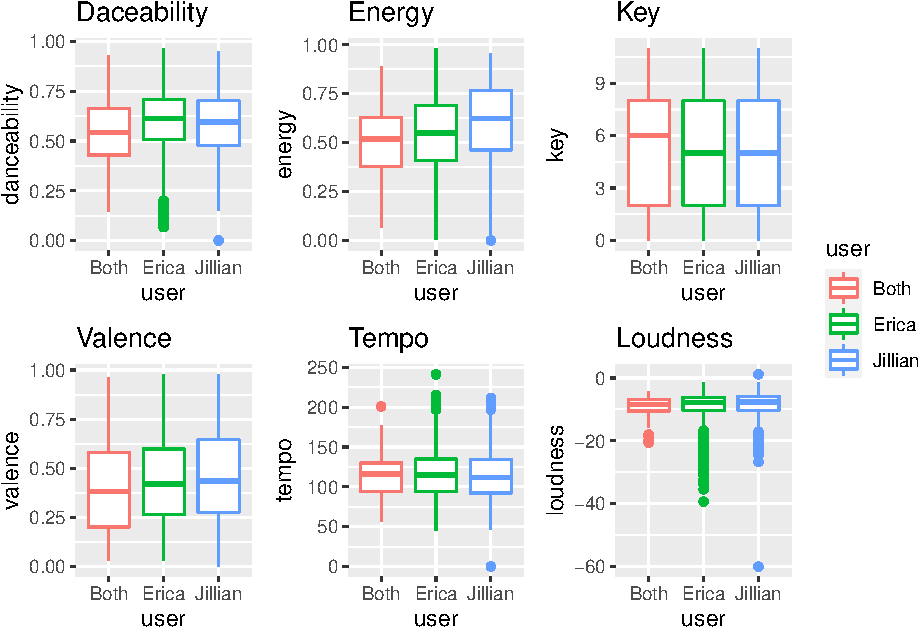
\includegraphics{Lab3_files/figure-latex/unnamed-chunk-4-1.pdf}

\begin{Shaded}
\begin{Highlighting}[]
\NormalTok{lasso\_cv }\OtherTok{\textless{}{-}} \FunctionTok{cv.glmnet}\NormalTok{(}\AttributeTok{x =}\NormalTok{ X,}
                       \AttributeTok{y =}\NormalTok{ Y,}
                       \AttributeTok{alpha =} \DecValTok{1}\NormalTok{)}

\NormalTok{lassocv\_plot }\OtherTok{\textless{}{-}} \FunctionTok{plot}\NormalTok{(lasso\_cv, }\AttributeTok{main =} \StringTok{"Lasso penalty}\SpecialCharTok{\textbackslash{}n\textbackslash{}n}\StringTok{"}\NormalTok{) }
\end{Highlighting}
\end{Shaded}

\includegraphics{Lab3_files/figure-latex/unnamed-chunk-4-2.pdf}

\begin{Shaded}
\begin{Highlighting}[]
\NormalTok{ ridgecv\_plot }
\end{Highlighting}
\end{Shaded}

\begin{verbatim}
## NULL
\end{verbatim}

\begin{Shaded}
\begin{Highlighting}[]
\NormalTok{ lassocv\_plot}
\end{Highlighting}
\end{Shaded}

\begin{verbatim}
## NULL
\end{verbatim}

\textbf{\emph{Question 5}}. Interpret the graphs. What is being show on
the axes here? How does the performance of the models change with the
value of lambda?

Both graphs show the mean squared error from the respective model
(showed by the red dots with gray bars indicated the confidence
interval). The vertical gray dotted lines show the log of \(\lambda\)
value correlated with the minimum mean-squared error (the first bar) and
the log of the \(\lambda\) value within one standard error of the
minimum MSE. The graphs use the log of \(\lambda\) to make it easier to
visualize the change in MSE in the model.

For the ridge regression plot, a \(Log(\lambda)\) value of around -1 to
-0.5 will minimize the error and therefore produce a better model. The
exact lambda values are calculated below. Ridge regressions do not
reduce the number of features, so all nine of the variables included in
the abalone data are included for each point calculated in the graph
above.

The lasso regression does reduce the number of features used from 9 to 5
(as shown in the upper horizontal axis). The MSE of the lasso model
starts to rapidly increase after a \(Log(\lambda)\) of about -2, and the
largest value within one standard error is about -3. This correlates
with a MSE of about 5, which is similar to the MSE produced by the ridge
model.

Because the MSE for the Lasso and Ridge regressions are similar, I would
recommend proceeding with the Lasso model that uses just five variables
instead of the ridge model that retains all nine features.

\textbf{\emph{Question 6}}. Inspect the ridge model object you created
with cv.glmnet(). The \$cvm column shows the MSEs for each cv fold. What
is the minimum MSE? What is the value of lambda associated with this MSE
minimum?

\begin{Shaded}
\begin{Highlighting}[]
\FunctionTok{print}\NormalTok{(ridge\_cv)}
\end{Highlighting}
\end{Shaded}

\begin{verbatim}
## 
## Call:  cv.glmnet(x = X, y = Y, alpha = 0) 
## 
## Measure: Mean-Squared Error 
## 
##     Lambda Index Measure     SE Nonzero
## min 0.2012   100   4.978 0.2116       9
## 1se 0.3516    94   5.168 0.2279       9
\end{verbatim}

\begin{Shaded}
\begin{Highlighting}[]
\FunctionTok{print}\NormalTok{(}\FunctionTok{paste}\NormalTok{(}\StringTok{"The minimum MSE for the ridege model is"}\NormalTok{, }\FunctionTok{round}\NormalTok{(}\FunctionTok{min}\NormalTok{(ridge\_cv}\SpecialCharTok{$}\NormalTok{cvm), }\DecValTok{2}\NormalTok{), }\StringTok{"and the corresponding lambda value is"}\NormalTok{, }\FunctionTok{round}\NormalTok{(ridge\_cv}\SpecialCharTok{$}\NormalTok{lambda.min, }\DecValTok{2}\NormalTok{)))}
\end{Highlighting}
\end{Shaded}

\begin{verbatim}
## [1] "The minimum MSE for the ridege model is 4.98 and the corresponding lambda value is 0.2"
\end{verbatim}

\textbf{\emph{Question 7}}. Do the same for the lasso model. What is the
minimum MSE? What is the value of lambda associated with this MSE
minimum?

\begin{Shaded}
\begin{Highlighting}[]
\FunctionTok{print}\NormalTok{(}\FunctionTok{paste}\NormalTok{(}\StringTok{"The minimum MSE for the lasso model is"}\NormalTok{, }\FunctionTok{round}\NormalTok{(}\FunctionTok{min}\NormalTok{(lasso\_cv}\SpecialCharTok{$}\NormalTok{cvm), }\DecValTok{2}\NormalTok{), }\StringTok{"and the corresponding lambda value is about"}\NormalTok{, }\FunctionTok{round}\NormalTok{(lasso\_cv}\SpecialCharTok{$}\NormalTok{lambda.min, }\DecValTok{3}\NormalTok{)))}
\end{Highlighting}
\end{Shaded}

\begin{verbatim}
## [1] "The minimum MSE for the lasso model is 4.65 and the corresponding lambda value is about 0.001"
\end{verbatim}

Data scientists often use the ``one-standard-error'' rule when tuning
lambda to select the best model. This rule tells us to pick the most
parsimonious model (fewest number of predictors) while still remaining
within one standard error of the overall minimum cross validation error.
The cv.glmnet() model object has a column that automatically finds the
value of lambda associated with the model that produces an MSE that is
one standard error from the MSE minimum (\$lambda.1se).

\begin{Shaded}
\begin{Highlighting}[]
\FunctionTok{print}\NormalTok{(}\FunctionTok{paste0}\NormalTok{(}\StringTok{"The lambda value within one standard error of the minimum MSE for the ridge model is "}\NormalTok{, }\FunctionTok{round}\NormalTok{(ridge\_cv}\SpecialCharTok{$}\NormalTok{lambda}\FloatTok{.1}\NormalTok{se, }\DecValTok{2}\NormalTok{), }\StringTok{", and the lambda value within one standard error of the overall minimum MSE for the lasso model is "}\NormalTok{, }\FunctionTok{round}\NormalTok{(lasso\_cv}\SpecialCharTok{$}\NormalTok{lambda}\FloatTok{.1}\NormalTok{se, }\DecValTok{2}\NormalTok{)))}
\end{Highlighting}
\end{Shaded}

\begin{verbatim}
## [1] "The lambda value within one standard error of the minimum MSE for the ridge model is 0.35, and the lambda value within one standard error of the overall minimum MSE for the lasso model is 0.06"
\end{verbatim}

\textbf{\emph{Question 8.}} Find the number of predictors associated
with this model (hint: the \$nzero is the \# of predictors column).

\begin{Shaded}
\begin{Highlighting}[]
\FunctionTok{print}\NormalTok{(}\FunctionTok{paste}\NormalTok{(}\StringTok{"The ridge model uses"}\NormalTok{, ridge\_cv}\SpecialCharTok{$}\NormalTok{nzero[ridge\_cv}\SpecialCharTok{$}\NormalTok{lambda }\SpecialCharTok{==}\NormalTok{ ridge\_cv}\SpecialCharTok{$}\NormalTok{lambda}\FloatTok{.1}\NormalTok{se], }\StringTok{"predictors."}\NormalTok{)) }\CommentTok{\#index to find where number of features corresponds to min lambda}
\end{Highlighting}
\end{Shaded}

\begin{verbatim}
## [1] "The ridge model uses 9 predictors."
\end{verbatim}

\begin{Shaded}
\begin{Highlighting}[]
\FunctionTok{print}\NormalTok{(}\FunctionTok{paste}\NormalTok{(}\StringTok{"The lasso model uses"}\NormalTok{, lasso\_cv}\SpecialCharTok{$}\NormalTok{nzero[lasso\_cv}\SpecialCharTok{$}\NormalTok{lambda }\SpecialCharTok{==}\NormalTok{ lasso\_cv}\SpecialCharTok{$}\NormalTok{lambda}\FloatTok{.1}\NormalTok{se], }\StringTok{"predictors."}\NormalTok{))}
\end{Highlighting}
\end{Shaded}

\begin{verbatim}
## [1] "The lasso model uses 5 predictors."
\end{verbatim}

\textbf{Question 9.} Which regularized regression worked better for this
task, ridge or lasso? Explain your answer.

Both models worked similarly for this task - coming up with similar MSE
values. However, because the lasso model had a slightly smaller MSE and
used fewer features, it would be the better model for this task.

\end{document}
